This section will go more into detail about the implementation we made and the design choices that were needed. 

\subsection{Flattening DBM}
In the \ltsmin{} implementation that we already have the state vector exists of all discrete variables and an 64 bit pointer to a C++ class containing a DBM~\cite{eemcs21972}. For a symbolic solution this pointer has no meaning, thus we take the actual values from the DBM and put these into the state vector. This increases the length of a state vector, but does not need to increase the memory footprint, as the DBM was already stored. 
In the DBM library we use a DBM is represented by a one dimensional array of 32-bit integers. In the integers the complete bound is stored, so both the operator and the constant value. We flattened the DBMs to work with a symbolic solution. We only did this on the edges of the successor function. So this function reads a flattened DBM as input and returns it as successor states, internally the original DBM representation is still used. This way the code had to be adapted the least. In this flattening we removed the diagonal elements of each DBM. By the way DBMs are constructed this will always represent the difference between a clock and itself. This difference is by definition always 0, so it can be removed, and hard coded be set to $(0,\leq)$ internally. This reduces the number of state variables in the state vector by one for each clock. This flattening of DBMs results into a language module that can be connected to all \ltsmin{} algorithmic back-ends for state-space generation. 

\subsection{Dependency Matrices}
To get the best possible result of the regrouping algorithms, the dependency matrices had to be made as sparse as possible. This has been done for both the read matrix and may-write matrix. For even better results, also the must-write matrix is needed. This needs effort when analysing the code, this can be done, but is left out for this thesis. First of all, all C-like code is parsed. Here it is stored per function which variables are read and written, and which other functions are called. Next all transitions are parsed, here some variables are read and written directly. Transitions can also call functions, in such cases the variables that were found in the parsing of these functions are added to the read and may-write variables of the transition. In the third step we need to look at the time extrapolation. This extrapolation is based on the value of the location variable, so it results in a read dependency. In some cases, there is no difference between all possible location values for this extrapolation, so a location does not need to be read. A final step is that a location variable that can be urgent or committed always has to be read. If this location is in an urgent state, than no other transitions can happen, so all other transitions have to check that they are not in an urgent state. In which only an other transition can take place.
The flattened DBMs and the sparser dependency matrices together enable the reordering algorithms in the symbolic back-end of \ltsmin{} to be used.

\subsection{DBM reduction}
We work towards a fully reduced DDD solution. This is already started at the language module size. The next-state function will only return tight and saturated paths. In DBM terms this is a minimal constraint system~\cite{bengtsson2002clocks}. As the length of a state-vector can not be changed on the fly, all removed constraints are set to $(<,\infty)$. This means that there is no upper-bound on the variable pair of that position. In algoorithm \ref{alg:ReduceZero} which uses algorithm \ref{alg:reduce} we show the algorithm that determines all bounds that are not needed an can be set to $(<,\infty)$. 
The DBM library can not use these minimal constraint systems. In the next state function the incoming DBM is tightened, then all needed operations for the successor generation are conducted and if a successor is returned, its DBM is again turned into a minimal constraint system. This will give algorithmic overhead for each next-state call. The advantage of this procedure is that many bounds will be redundant and turned into $(<,\infty)$. In the symbolic back-end these bounds which are the same can be shared in a single node. Thus taking more time in the successor generator, it can also reduce the number of nodes in the algorithmic back-end.
This reduction is used in the successor generator for the symbolic back-end, and will also be used for the DDD solution.

\begin{algorithm}
\caption{Reduce}\label{alg:Reduce}
\begin{algorithmic}[1]
\Procedure{Reduce}{$dbm, dim$}
	\For{$i \in dim$}
		\For{$j \in dim$}
			\For{$k \in dim$}
				\If{$!(dbm[i,k] \vee dbm[k,j] \vee dbm[i,j]$ on diagonal)}
					\If{$dbm[i,k] + dbm[k,j] \leq dbm[i,j]$}
						\State{$dbm[i,j] := \infty$} 
					\EndIf
				\EndIf
			\EndFor
		\EndFor
	\EndFor				
\EndProcedure
\end{algorithmic}
\end{algorithm}

\begin{algorithm}
\caption{Reduce}\label{alg:ReduceZero}
\begin{algorithmic}[1]
\Procedure{ReduceZero}{$dbm, dim$}
	\State{$placed[dim]$ all 0}
	\State{$red[dim,dim]$ all 0}
	\State{$eq[dim,dim]$ all 0}
	\State{$cl := 0$}
	\State{$newDBM[dim,dim]$ diagonal $\infty$ rest $0$}
	\For{$i \in dim$}
		\If{$placed[i] = 0$}
			\For{$j \in \dim$}
				\If{$dbm[i,j] + dbm[j,i] = 0$}
					\State{$placed[j] := 1$}
					\State{$eq[cl,j] := 1$}
				\EndIf
			\EndFor
			\State{$cl++$}
		\EndIf
	\EndFor
	\State{$repr[cl]$}
	\For{$i \in cl$}
		\For{$j \in dim$}
			\If{$eq[i,j] = 1$}
				\State{$repr[i] := j$}
				\Break
			\EndIf
		\EndFor
	\EndFor
	\State{$clg[cl,cl]$}
	\For{$i \in cl$}
		\For{$j \in cl$}
			\State{$clg[i,j] := dbm[repr[i],repr[j]]$}
		\EndFor
	\EndFor
	\State{\Call{Reduce}{$clg, cl$}}
	\For{$i \in cl$}
		\For{$j \in dim$}
			\If{$eq[i,j] = 1$}
				\For{$k \in dim$}
					\If{$eq[i,k]$}
						\State{$newDBM[j,k] = dbm[j,k]$}
					\EndIf
				\EndFor
			\EndIf
		\EndFor
		\For{$j \in cl$}
			\State{$newDBM[repr[i],repr[j]] := clg[i,j]$}
		\EndFor
	\EndFor
	\State{\Return newDBM}
		
\EndProcedure
\end{algorithmic}
\end{algorithm}

\subsection{Connecting LDD and DDD}
To represent the discrete variables in states LDD nodes are used. The structure of these nodes is quite similar to DDD nodes. We decided to not mix the nodes, but to first have all the LDD nodes and then all DDD nodes in the tree. In the state vector the first part exists of all discrete variables, the last part are the DBM variables. The top of the diagram can be seen as a MTLDD(Multi-Terminal List Decision Diagram) with not values on the leaf nodes, but pointers to DDD nodes. The DDD part is not influenced by the LDD part, as a node is only influenced by the nodes below it, it has no information about the nodes above it in the diagram. This strict separation between LDD and DDD nodes makes that the reordering algorithms can not be used. The lack of reordering makes it also possible to reconstruct the DBMs on the DDD side. This is used for the minus function which we discuss later.

\subsection{DDD nodes}
We used the basis of the LDD package in Sylvan to create our DDD nodes. The nodes are the same as the LDD nodes, only two previously unused bits are now used to store the operator and the type of the node. DDD nodes are stored in 128 bits, represented as a struct of two 64 bit integers. The hashtable that is already used by Sylvan is specifically for 128 bit entries, so the DDD nodes can use the same hashtable. A node is in C code represented as follows:
\begin{lstlisting} 

struct dddnode {
    uint64_t a, b;
} * dddnode_t; 
\end{lstlisting}

In this struct the value(32 bits), the true edge(40 bits), the false edge(40 bits) and a type bit, operator bit and flag bit are stored. These values are not specifically named in the struct, all values are stored in the two integers a and b. Figure \ref{fig:ddd-node} shows how this is coded in memory. The type, operator and flag bit are stored in the black areas. We do not show them explicitly due to the scale.
The type bit indicates if a node is a DDD or an LDD node, if it is set to 0 it should be treated as a normal LDD node. The operator bit shows if the operator is $<$ or $\leq$, this can only be used if the type bit is also set to 1(DDD). The flag bit is used in some algorithms to indicate that a certain node has already been visited. All of this is stored compactly in the two 64 bit integers. The total information is 115 bits, so there are still 17 unused bits, all unused bits are set to 0. The depth of the node is not stored, this can be calculated by going down through the structure. This implies that no level can be skipped. Other DDD algorithms and reductions show that some levels are not needed. We solved this by indication a skipped level by $< \infty$, which is true for every upper bound. For such nodes the false edge will always directly lead to the false end node.

\begin{figure}
\centering
\begin{bytefield}[bitwidth=1.2em]{16}
  \bitbox{5}{low edge}
  \bitbox{1}{\rule{\width}{\height}}
  \bitbox{4}{value}
  \bitbox{1}{\rule{\width}{\height}}
  \bitbox{5}{high edge}\\
\end{bytefield}
\caption{In memory representation of DDD node}
\label{fig:ddd-node}
\end{figure}

\subsection{Creating Nodes}
To create a node a special MK function is used. This function will ensure that a DDD is always locally reduced. This MK function is shown in algorithm \ref{alg:MK}. This function ensures the correct total structure and puts newly created nodes in the hashtable. The actual creation of a node is done in the MakeNode function that is called inside the MK function. The code for the MakeNode function is not shown here as it is only technical coding, putting all the information in the struct.
\begin{algorithm}
\caption{MK}\label{alg:MK}
\begin{algorithmic}[1]
\Procedure{MK}{$value, h, l, type, op$}
	\If{$h = 0 \wedge type = LDD$}
		\State \Return $l$
	\EndIf
	\If{$h = 1 \wedge l = 1$}
		\State \Return $1$
	\EndIf
	\If{$h = 0 \wedge l = 0$}
		\State \Return $0$
	\EndIf
	\If{$h = 0 \wedge l \neq 0$}
		\State \Return $1$
	\EndIf
	\If{$h = high(l)$}
		\State \Return $l$
	\EndIf
	\State $node =$ \Call{makeNode}{$value, h, l, type, op$}
	\If{$node \notin table$}
		\State \Call{Put}{$node$}
	\EndIf
	\State \Return $node$
\EndProcedure	
\end{algorithmic}
\end{algorithm}

%\begin{algorithm}
%\caption{MakeNode}\label{alg:MakeNode}
%\begin{algorithmic}[1]
%\Procedure{MakeNode}{$value, h, l, type, op$}
%	\State $dddnode_t n$
%	\State $n->a := l << 1$
%	\State{ $n->b := h << 17$}
%    \State $n->a := (n->a & 0xffffbfffffffffff) | (op << 46)$
%	\State $n->a := (n->a & 0xffffbfffffffffff) | (type << 47)$
%	\State $*(int32_t*)((uint8_t*)n+6) := value$
%\EndProcedure	
%\end{algorithmic}
%\end{algorithm}

\subsection{Apply}
One of the core operations on DDDs is the apply operation. This operation takes two DDDs and a binary operator and combines the two DDDs according to the operator. The apply function for DDDs is a generalisation of the function for BDDs. In ~\cite{ddds} a general definition of the algorithm is given. We turned this more mathematical definition into an algorithm, we give pseudo-code in Algorithm \ref{alg:apply}. The algorithm will search down to the leaf nodes and use the operator on that level. We can optimize this a bit for cases where we see two equal nodes, or only one leaf node. In Algorithm \ref{alg:union} we give the pseudo-code for the apply function with the or operator, or the union function, this way we can increase performance by not going down the entire diagram if we already found a false leaf, or two equal nodes. The apply operator does not ensure path-reducedness, even when both inputs are path reduced. 

\begin{algorithm}
\begin{algorithmic}[1]
\caption{Apply}\label{alg:apply}
\Procedure{Apply}{$v1, v2, op$}
	\If{$v1 \in \{0,1\} \wedge v2 \in \{0,1\}$}
		\State $result \gets (v1$ $op$ $v2)$
	\ElsIf{$var(v1) \prec var(v2)$}
		\State $high \gets$ \Call{Apply}{$high(v1), v2, op$}
		\State $low \gets$ \Call{Apply}{$low(v1), v2, op$}
		\State $result \gets$ \Call{Mk}{$cstr(v1), high, low$} 
	\ElsIf{$var(v2) \prec var(v1)$}
		\State $high \gets$ \Call{Apply}{$high(v2), v1, op$}
		\State $low \gets$ \Call{Apply}{$low(v2), v1, op$}
		\State $result \gets$ \Call{Mk}{$cstr(v2), high, low$} 
	\ElsIf{$v1 \prec v2$}
		\State $high \gets$ \Call{Apply}{$high(v1), high(v2), op$}
		\State $low \gets$ \Call{Apply}{$low(v1), v2, op$}
		\State $result \gets$ \Call{Mk}{$cstr(v1), high, low$}
	\ElsIf{$v2 \prec v1$}
		\State $high \gets$ \Call{Apply}{$high(v1), high(v2), op$}
		\State $low \gets$ \Call{Apply}{$v1, low(v2), op$}
		\State $result \gets$ \Call{Mk}{$cstr(v2), high, low$}
	\ElsIf{$v1 = v2$}
		\State $high(v1) \gets$ \Call{Apply}{$high(v1), high(v2), op$}
		\State $low(v1) \gets$ \Call{Apply}{$low(v1), low(v2), op$}
		\State $result \gets$ \Call{Mk}{$cstr(v1), high, low$}
	\EndIf
	\State \Return $result$
\EndProcedure
\end{algorithmic}
\end{algorithm}

\begin{algorithm}
\begin{algorithmic}[1]
\caption{Union}\label{alg:union}
\Procedure{Union}{$v1, v2$}
	\If{$v1 = v2$} 
		\Return{$v1$} 
	\ElsIf{$v1 =$ \False}
		\Return{$v2$}
	\ElsIf{$v2 =$ \False}
		\Return{$v1$}
	\ElsIf{$var(v1) \prec var(v2)$}
		\State $high \gets$ \Call{Union}{$high(v1), v2$}
		\State $low \gets$ \Call{Union}{$low(v1), v2$}
		\State $result \gets$ \Call{Mk}{$cstr(v1), high, low$} 
	\ElsIf{$var(v2) \prec var(v1)$}
		\State $high \gets$ \Call{Union}{$high(v2), v1$}
		\State $low \gets$ \Call{Union}{$low(v2), v1$}
		\State $result \gets$ \Call{Mk}{$cstr(v2), high, low$} 
	\ElsIf{$v1 \prec v2$}
		\State $high \gets$ \Call{Union}{$high(v1), high(v2)$}
		\State $low \gets$ \Call{Union}{$low(v1), v2$}
		\State $result \gets$ \Call{Mk}{$cstr(v1), high, low$}
	\ElsIf{$v2 \prec v1$}
		\State $high \gets$ \Call{Union}{$high(v1), high(v2)$}
		\State $low \gets$ \Call{Union}{$v1, low(v2)$}
		\State $result \gets$ \Call{Mk}{$cstr(v2), high, low$}
	\ElsIf{$v1 = v2$}
		\State $high(v1) \gets$ \Call{Union}{$high(v1), high(v2)$}
		\State $low(v1) \gets$ \Call{Union}{$low(v1), low(v2)$}
		\State $result \gets$ \Call{Mk}{$cstr(v1), high, low$}
	\EndIf
	\State \Return $result$
\EndProcedure
\end{algorithmic}
\end{algorithm}

\subsection{Minus}
The minus function, used for the reachability, has not been implemented as an DDD functions. This function is different to other functions, as information has to be transferred over different levels. For simple cases, an upper-bound in one of the operands of the minus, can become a lower-bound in the result, and vice-versa. A simple one dimensional example is $[0..8] / [0..4)$, this will result in $[4..8]$. In this case the 4 is the upper-bound of the subtrahend. It will however become the lower-bound of the difference. As lower- and upper-bounds are saved on different levels in DDDs this makes the function different from all other functions, which only look at values on the same level.

In figure \ref{fig:md-minus} we have a two-dimensional example of how the minus function can become more complex for multiple-dimensions. In this case we make a hole in a larger zone. Both the minuend and the subtrahend are represented by a DDD with a single path, as shown in figure \ref{fig:difference-ddd}. For simplicity we removed the diagonals in this example, as they play no role. The difference however becomes a DDD with 4 paths and 10 nodes, figure \ref{fig:difference-ddd-res}. Again a lot of upper- and lower-bounds are switched. Already for this example we could not find a algorithm that does this in general. For more dimensions, and DDDs with already multiple paths the problem will only get harder. That is why we returned to a DBM function for this.

\begin{figure}[h]

\begin{subfigure}[b]{\textwidth}
\centering
\begin{adjustbox}{max totalheight=.3\textheight}
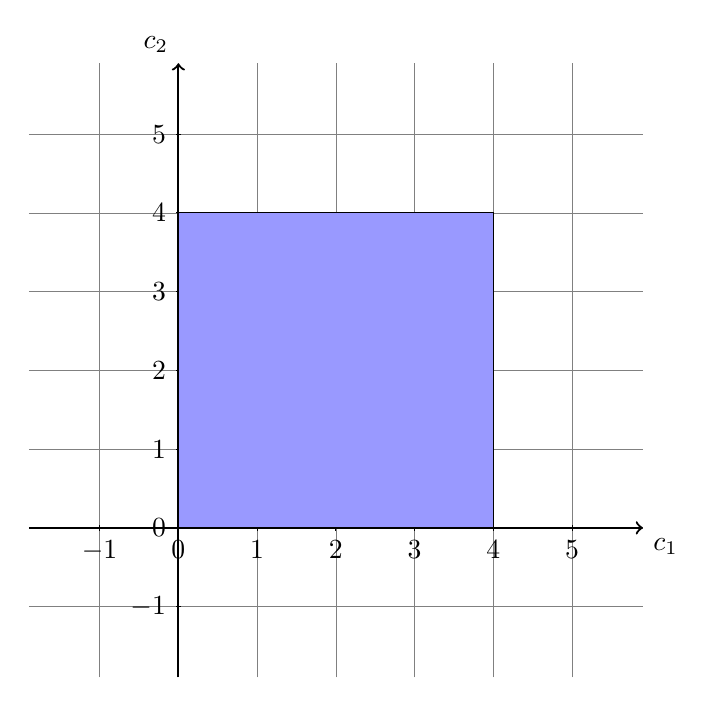
\begin{tikzpicture}

\draw[step=1cm,gray,very thin] (-1.9,-1.9) grid (5.9,5.9);

%\shadedraw[inner color=blue,outer color=red, draw=black] (0,0) rectangle (4,4);

\draw[thick,->] (-1.9,0) -- (5.9,0) node[anchor=north west] {$c_1$};
\draw[thick,->] (0,-1.9) -- (0,5.9) node[anchor=south east] {$c_2$};

\foreach \x in {-1,0,1,2,3,4,5}
    \draw (\x cm,1pt) -- (\x cm,-1pt) node[anchor=north] {$\x$};
\foreach \y in {-1,0,1,2,3,4,5}
    \draw (1pt,\y cm) -- (-1pt,\y cm) node[anchor=east] {$\y$};
    
\filldraw[fill=blue!40!white, draw=black] (0,0) rectangle (4,4);

\end{tikzpicture}
\end{adjustbox}
\caption{Minuend}
\label{fig:minuend_zone}
\end{subfigure}

\begin{subfigure}[b]{\textwidth}
\centering
\begin{adjustbox}{max totalheight=.3\textheight}
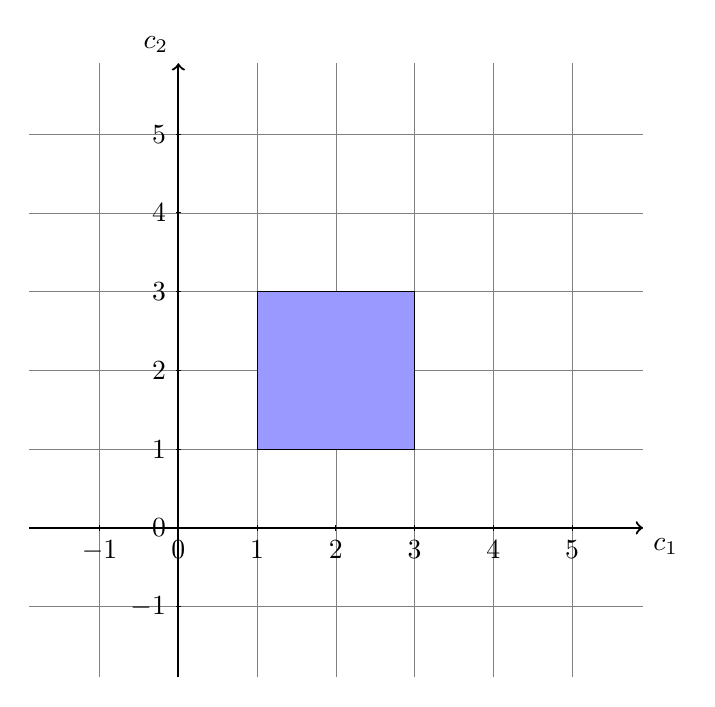
\begin{tikzpicture}
\draw[step=1cm,gray,very thin] (-1.9,-1.9) grid (5.9,5.9);

%\shadedraw[inner color=blue,outer color=red, draw=black] (0,0) rectangle (4,4);

\draw[thick,->] (-1.9,0) -- (5.9,0) node[anchor=north west] {$c_1$};
\draw[thick,->] (0,-1.9) -- (0,5.9) node[anchor=south east] {$c_2$};

\foreach \x in {-1,0,1,2,3,4,5}
    \draw (\x cm,1pt) -- (\x cm,-1pt) node[anchor=north] {$\x$};
\foreach \y in {-1,0,1,2,3,4,5}
    \draw (1pt,\y cm) -- (-1pt,\y cm) node[anchor=east] {$\y$};
    
\filldraw[fill=blue!40!white, draw=black] (1,1) rectangle (3,3);

\end{tikzpicture}
\end{adjustbox}
\caption{Subtrahend}
\label{fig:subtrahend_zone}
\end{subfigure}




\begin{subfigure}[b]{\textwidth}
\centering
\begin{adjustbox}{max totalheight=.3\textheight}
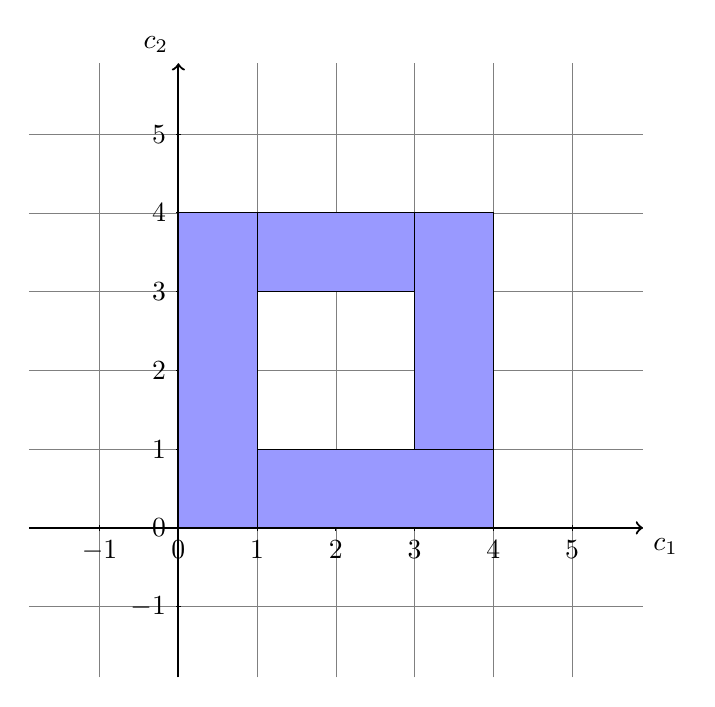
\begin{tikzpicture}
\draw[step=1cm,gray,very thin] (-1.9,-1.9) grid (5.9,5.9);

%\shadedraw[inner color=blue,outer color=red, draw=black] (0,0) rectangle (4,4);

\draw[thick,->] (-1.9,0) -- (5.9,0) node[anchor=north west] {$c_1$};
\draw[thick,->] (0,-1.9) -- (0,5.9) node[anchor=south east] {$c_2$};

\foreach \x in {-1,0,1,2,3,4,5}
    \draw (\x cm,1pt) -- (\x cm,-1pt) node[anchor=north] {$\x$};
\foreach \y in {-1,0,1,2,3,4,5}
    \draw (1pt,\y cm) -- (-1pt,\y cm) node[anchor=east] {$\y$};
    
\filldraw[fill=blue!40!white, draw=black] (0,3) rectangle (4,4);
\filldraw[fill=blue!40!white, draw=black] (3,0) rectangle (4,4);
\filldraw[fill=blue!40!white, draw=black] (0,0) rectangle (4,1);
\filldraw[fill=blue!40!white, draw=black] (0,0) rectangle (1,4);

\end{tikzpicture}
\end{adjustbox}
\caption{Difference}
\label{fig:difference_zone}
\end{subfigure}

\caption{Minus complexity example}
\label{fig:md-minus}
\end{figure}

\begin{figure}[h]
\begin{center}
	\begin{subfigure}{0.3\textwidth}
	\begin{tikzpicture}[
		smallvertex/.style={circle,draw,scale=0.8}
		]
		\node[smallvertex, draw = none, above of = S1, yshift = 0.25cm](S0){};
		\node[smallvertex](S1){$\mathbf{O} - c_1$};
		\node[smallvertex, below of = S1, yshift = -1cm](S2){$\mathbf{O} - c_2$};
		\node[smallvertex, below of = S2, yshift = -1cm](S3){$c_1 - \mathbf{O}$};
		\node[smallvertex, below of = S3, yshift = -1cm](S4){$c_2 - \mathbf{O}$};
		\node[smallvertex, below of = S4, yshift = -1cm](S5){$T$};
		
		\draw[->] (S0) --(S1) node [midway, above, sloped, scale=0.75,
		rotate=0, xshift =-0.4 cm, yshift = -0.2cm]{};
		\draw[->] (S1) --(S2) node [midway, above, sloped, scale=0.75,
		rotate=90, xshift =-0.4 cm, yshift = -0.2cm]{$<0$};
		\draw[->] (S2) --(S3) node [midway, above, sloped, scale=0.75,
		rotate=90, xshift =-0.4 cm, yshift = -0.2cm]{$<0$};
		\draw[->] (S3) --(S4) node [midway, above, sloped, scale=0.75,
		rotate=90, xshift =-0.4 cm, yshift = -0.2cm]{$<4$};
		\draw[->] (S4) --(S5) node [midway, above, sloped, scale=0.75,
		rotate=90, xshift =-0.4 cm, yshift = -0.2cm]{$<4$};

	\end{tikzpicture}
	\end{subfigure}
	\begin{subfigure}{0.3\textwidth}
	\begin{tikzpicture}[
		smallvertex/.style={circle,draw,scale=0.8}
		]
		\node[smallvertex, draw = none, above of = S1, yshift = 0.25cm](S0){};
		\node[smallvertex](S1){$\mathbf{O} - c_1$};
		\node[smallvertex, below of = S1, yshift = -1cm](S2){$\mathbf{O} - c_2$};
		\node[smallvertex, below of = S2, yshift = -1cm](S3){$c_1 - \mathbf{O}$};
		\node[smallvertex, below of = S3, yshift = -1cm](S4){$c_2 - \mathbf{O}$};
		\node[smallvertex, below of = S4, yshift = -1cm](S5){$T$};
		
		\draw[->] (S0) --(S1) node [midway, above, sloped, scale=0.75,
		rotate=0, xshift =-0.4 cm, yshift = -0.2cm]{};
		\draw[->] (S1) --(S2) node [midway, above, sloped, scale=0.75,
		rotate=90, xshift =-0.4 cm, yshift = -0.2cm]{$<-1$};
		\draw[->] (S2) --(S3) node [midway, above, sloped, scale=0.75,
		rotate=90, xshift =-0.4 cm, yshift = -0.2cm]{$<-1$};
		\draw[->] (S3) --(S4) node [midway, above, sloped, scale=0.75,
		rotate=90, xshift =-0.4 cm, yshift = -0.2cm]{$<3$};
		\draw[->] (S4) --(S5) node [midway, above, sloped, scale=0.75,
		rotate=90, xshift =-0.4 cm, yshift = -0.2cm]{$<3$};
		
	\end{tikzpicture}
	\end{subfigure}
\end{center}
\caption{DDD representation of the minuend and subtrahend of figure \ref{fig:md-minus}}
\label{fig:difference-ddd}
\end{figure}

\begin{figure}[h]
\begin{center}
	\begin{tikzpicture}[
		smallvertex/.style={circle,draw,scale=0.8}
		]
		\node[smallvertex, draw = none, above of = S1, yshift = 0.25cm](S0){};
		\node[smallvertex](S1){$\mathbf{O} - c_1$};
		\node[smallvertex, below of = S1, yshift = -1cm](S2){$\mathbf{O} - c_2$};
		\node[smallvertex, below of = S2, yshift = -1cm](S3){$c_1 - \mathbf{O}$};
		\node[smallvertex, below of = S3, yshift = -1cm](S4){$c_2 - \mathbf{O}$};
		\node[smallvertex, below of = S4, yshift = -1cm](S5){$T$};
		\node[smallvertex, right of = S1, xshift = 1cm](S6){$\mathbf{O} - c_1$};
		\node[smallvertex, below of = S6, yshift = -1cm](S7){$\mathbf{O} - c_2$};
		\node[smallvertex, right of = S7, xshift = 1cm](S8){$\mathbf{O} - c_2$};
		\node[smallvertex, below of = S8, yshift = -1cm](S9){$c_1 - \mathbf{O}$};
		\node[smallvertex, right of = S9, xshift = 1cm](S10){$c_1 - \mathbf{O}$};
		\node[smallvertex, below of = S10, yshift = -1cm](S11){$c_2 - \mathbf{O}$};
		
		
		\draw[->] (S0) --(S1) node [midway, above, sloped, scale=0.75,
		rotate=0, xshift =-0.4 cm, yshift = -0.2cm]{};
		\draw[->] (S1) --(S2) node [midway, above, sloped, scale=0.75,
		rotate=90, xshift =-0.4 cm, yshift = -0.2cm]{$\leq1$};
		\draw[->] (S2) --(S3) node [midway, above, sloped, scale=0.75,
		rotate=90, xshift =-0.4 cm, yshift = -0.2cm]{$<0$};
		\draw[->] (S3) --(S4) node [midway, above, sloped, scale=0.75,
		rotate=90, xshift =-0.4 cm, yshift = -0.2cm]{$<4$};
		\draw[->] (S4) --(S5) node [midway, above, sloped, scale=0.75,
		rotate=90, xshift =-0.4 cm, yshift = -0.2cm]{$<0$};
		\draw[dashed,->] (S1) --(S6) node [midway, above, sloped, scale=0.75,
		rotate=0, xshift =-0.7 cm, yshift = -0.2cm]{};
		\draw[->] (S6) --(S7) node [midway, above, sloped, scale=0.75,
		rotate=90, xshift =-0.4 cm, yshift = -0.2cm]{$<4$};
		\draw[->] (S7) --(S3) node [midway, above, sloped, scale=0.75,
		rotate=315, xshift =-0.4 cm, yshift = -0.2cm]{$\leq-3$};
		\draw[dashed,->] (S7) --(S8) node [midway, above, sloped, scale=0.75,
		rotate=0, xshift =-0.7 cm, yshift = -0.2cm]{};
		\draw[->] (S8) --(S9) node [midway, above, sloped, scale=0.75,
		rotate=90, xshift =-0.4 cm, yshift = -0.2cm]{$<0$};
		\draw[->] (S9) --(S4) node [midway, above, sloped, scale=0.75,
		rotate=335, xshift =-0.4 cm, yshift = -0.2cm]{$\leq1$};
		\draw[dashed,->] (S9) --(S10) node [midway, above, sloped, scale=0.75,
		rotate=0, xshift =-0.7 cm, yshift = -0.2cm]{};
		\draw[->] (S10) --(S11) node [midway, above, sloped, scale=0.75,
		rotate=90, xshift =-0.4 cm, yshift = -0.2cm]{$<4$};
		\draw[->] (S11) --(S5) node [midway, above, sloped, scale=0.75,
		rotate=340, xshift =-0.4 cm, yshift = -0.2cm]{$\leq-3$};

	\end{tikzpicture}
\end{center}
\caption{DDD representation of the difference of figure \ref{fig:md-minus}}
\label{fig:difference-ddd-res}
\end{figure}

The DBM function we use is defined in the \uppaal{} DBM library. The minus function is defined over a federation of DBMs. This federation is a C++ class containing multiple DBMs. This federation is needed as we can do a minus over a collection of zones, multiple paths in the DDD, and the result can contain multiple zones. As already shown in the example of figure \ref{fig:md-minus}. For this function we first take the normal LDD minus function over the discrete part. At the first DDD level, representing the zones, the DBM function is called. From this level all possible paths are searched, and for each path a DBM is created and tightened. All these DBMs are put in a federation, on which the library function can be called. The result is again (a possibly empty) federation. If the federation is empty, simply a DDD-false node is returned. Otherwise each DBM is turned into a DDD path and these paths are made into a single structure using the union function.

\subsection{BFS}
\label{subsection:bfs}
The DBM minus function we use is quite expensive. As it is imported from a library we do not know the exact complexity. To overcome this problem we will use two different versions of the search algorithm. Our second version will not use the minus function. In algorithm \ref{alg:bfs-orig} we show the standard BFS algorithm, this will be the first algorithm we use. Algorithm \ref{alg:bfs-check} shows how we can edit this algorithm. The constraint of the loop is changed from an empty check of the current set, to a check that the total visited set has not been changed. This check is basically the same, the first checks if now new states are found, the second checks that the total state-space has not been changed. This change now shows that the minus is not necessary any more, as shown in algorithm \ref{alg:bfs-no-minus}. This version uses the same check as the previous one, but now the minus of the current and the visited set has been removed. The implication is that the current set will in some cases be larger than in the previous algorithm. This will have some negative impact on the next-state calls, which will take more time. Not using the expensive minus function might compensate for that. We have implemented these two versions in the bfs-prev algorithm~\cite{rwcmatrices}. This is the default search algorithm that is used in \ltsmin{}. In the results section we will show the outcome of both BFS algorithms. 

\begin{algorithm}
\caption{BFS}\label{alg:bfs-orig}
\begin{algorithmic}[1]
\Procedure{BFS}{$initial$}
	\State $vis := cur := initial$
	\While{$cur \neq \emptyset$}
		\State{$cur := next(cur)$}
		\State{$vis := vis \cup cur$}
		\State{$cur := cur \setminus vis$}
	\EndWhile
	
\EndProcedure	
\end{algorithmic}
\end{algorithm}

\begin{algorithm}
\caption{BFS}\label{alg:bfs-check}
\begin{algorithmic}[1]
\Procedure{BFS}{$initial$}
	\State $vis := cur := initial$
	\State $vis_{prev} := \emptyset$
	\While{$vis \neq vis_{prev}$}
		\State{$vis_{prev} := vis$}
		\State{$cur := next(cur)$}
		\State{$vis := vis \cup cur$}
		\State{$cur := cur \setminus vis$}
	\EndWhile
	
\EndProcedure	
\end{algorithmic}
\end{algorithm}

\begin{algorithm}
\caption{BFS}\label{alg:bfs-no-minus}
\begin{algorithmic}[1]
\Procedure{BFS}{$initial$}
	\State $vis := cur := initial$
	\State $vis_{prev} := \emptyset$
	\While{$vis \neq vis_{prev}$}
		\State{$vis_{prev} := vis$}
		\State{$cur := next(cur)$}
		\State{$vis := vis \cup cur$}
	\EndWhile
	
\EndProcedure	
\end{algorithmic}
\end{algorithm}
